\documentclass[12pt,aspectratio=169,handout]{beamer}
\usepackage[utf8]{vietnam}
\usepackage{algorithm}
\usepackage{algorithmic}
\usepackage{indentfirst}
\usepackage{tikz}
\usepackage{pgfplots}
\usepackage{graphicx}
\usepackage{float}
\usepackage{subfig}

\usepackage{listings}
\usepackage{xcolor}

\definecolor{codegreen}{rgb}{0,0.6,0}
\definecolor{codegray}{rgb}{0.5,0.5,0.5}
\definecolor{codepurple}{rgb}{0.58,0,0.82}
\definecolor{backcolour}{rgb}{0.95,0.95,0.92}

\lstdefinestyle{mystyle}{
    backgroundcolor=\color{backcolour},   
    commentstyle=\color{codegreen},
    keywordstyle=\color{magenta},
    numberstyle=\tiny\color{codegray},
    stringstyle=\color{codepurple},
    basicstyle=\ttfamily\footnotesize,
    breakatwhitespace=false,         
    breaklines=true,                 
    captionpos=b,                    
    keepspaces=true,                 
    numbers=left,                    
    numbersep=5pt,                  
    showspaces=false,                
    showstringspaces=false,
    showtabs=false,                  
    tabsize=2
}

\lstset{style=mystyle}

\usepackage{amsfonts, amsmath, amssymb, amsthm}
\title[HTQL Light Novel]{Hệ thống quản lý Light Novel}
\subtitle{Project môn học: Thực hành CSDL}
\author{Nhóm 1}
\institute{Đại học Bách Khoa Hà Nội}

\usetheme{CambridgeUS}
\usecolortheme{dolphin}
\usefonttheme{structurebold} %
\begin{document}
\titlepage

\begin{frame}{Nội dung}
    \tableofcontents[pausesections]
\end{frame}

\AtBeginSection[]{
    \begin{frame}{Nội dung}
        \tableofcontents[currentsection]
    \end{frame}
}

% yêu cầu mô tả rõ hơn
% chuẩn hóa
% thêm thực thể: 
\section{Mô tả bài toán}
\begin{frame}{Mục tiêu}
    Xây dựng một hệ thống web cho phép người dùng đọc light novel, tiếp cận với những bộ truyện mới nhất, và có thể bình luận về các bộ truyện mà mình đã đọc.
    \begin{block}{Yêu cầu hệ thống}
        Người dùng có thể:
        \begin{itemize}
            \item Xem tổng quan về các bộ light novel, bao gồm tên, tác giả, thể loại, mô tả, ảnh bìa, đánh giá, trạng thái (đang ra hay đã hoàn thành), tóm tắt nội dung, thời gian cập nhật gần nhất và thời gian tạo.
            \item Xem danh sách các chương của một bộ light novel, bao gồm tên chương, thời gian xuất bản và nội dung.
            \item Đọc các chương của bộ light novel.
            \item Đưa ra đánh giá và bình luận cho bộ novel đó.
        \end{itemize}
    \end{block}
\end{frame}

\begin{frame}{Yêu cầu hệ thống (continued)}
    \begin{block}{Đối với tác giả}
        Tác giả có thể:
        \begin{itemize}
            \item Thêm và sửa đổi các thuộc tính như thể loại, mô tả, trạng thái của một LN mình viết 
            \item Tạo và chỉnh sửa các chương của một LN 
        \end{itemize}
    \end{block}
    \pause
    \begin{block}{Đối với người quản trị}
        \begin{itemize}
            \item Có thể thêm và xoá các tác giả, LNs và thể loại
            \item Quản lý đánh giá (chỉ có thể xoá hoặc ẩn, không thể chỉnh sửa nội dung!)
        \end{itemize}
    \end{block}
\end{frame}

% \begin{frame}{Yêu cầu phi chức năng}
% 	\begin{itemize}
% 		\item Tính bảo mật
%         \item Phù hợp với người dùng (được viết bằng HTML/CSS để dễ tiếp cận)
%     \end{itemize}
% \end{frame}

\section{Thiết kế cơ sở dữ liệu}

\begin{frame}
    \frametitle{Các thực thể}
    \begin{itemize}
        \item \textbf{User}(\underline{user\_id}, username, password, role, created\_at, ...)
        \item \textbf{Author}(\underline{author\_id}, author\_name, description, profile\_picture)
        \item \textbf{Novel}(\underline{novel\_id}, name, author, genre, description, cover, status, last\_updated, created\_at)
        \item \textbf{Genre}(\underline{genre\_id}, genre\_name, genre\_description)
        \item \textbf{Chapter}(\underline{chapter\_id}, novel\_id (fk), chapter\_number, title, published\_date, content)
        % \item \textbf{Comment}(\underline{comment\_id}, user\_id (fk), novel\_id (fk), content, is\_visible, created\_at)
        \item \textbf{Rating}(\underline{rating\_id}, user\_id (fk), novel\_id (fk), stars, content, created\_at)
    \end{itemize}
\end{frame}

\begin{frame}
    \frametitle{Mối quan hệ}
    \begin{itemize}
        \item Một bộ light novel có thể có nhiều chương.
        \item Một bộ light novel có thể thuộc nhiều thể loại.
        \item Một bộ light novel có thể có nhiều tác giả.
        % \item Một bình luận thuộc về một người dùng và một bộ light novel.
        \item Một đánh giá thuộc về một người dùng và một bộ light novel.
    \end{itemize}
\end{frame}

\begin{frame}
	\frametitle{Liên kết giữa các thực thể}
	\begin{center}
		\begin{tabular}{|c|c|}
			\hline
			\textbf{Thực thể} & \textbf{Liên kết} \\
			\hline
			Novel - Chapter & 1 - N \\
			Novel - Genre & N - N \\
			Novel - Author & N - N \\
			% Novel - Comment & 1 - N \\
			Novel - Rating & 1 - N \\
			% User - Comment & 1 - N \\
			User - Rating & 1 - N \\
			\hline
		\end{tabular}
	\end{center}
\end{frame}


\begin{frame}
    \frametitle{Sơ đồ ER}
    \begin{center}
        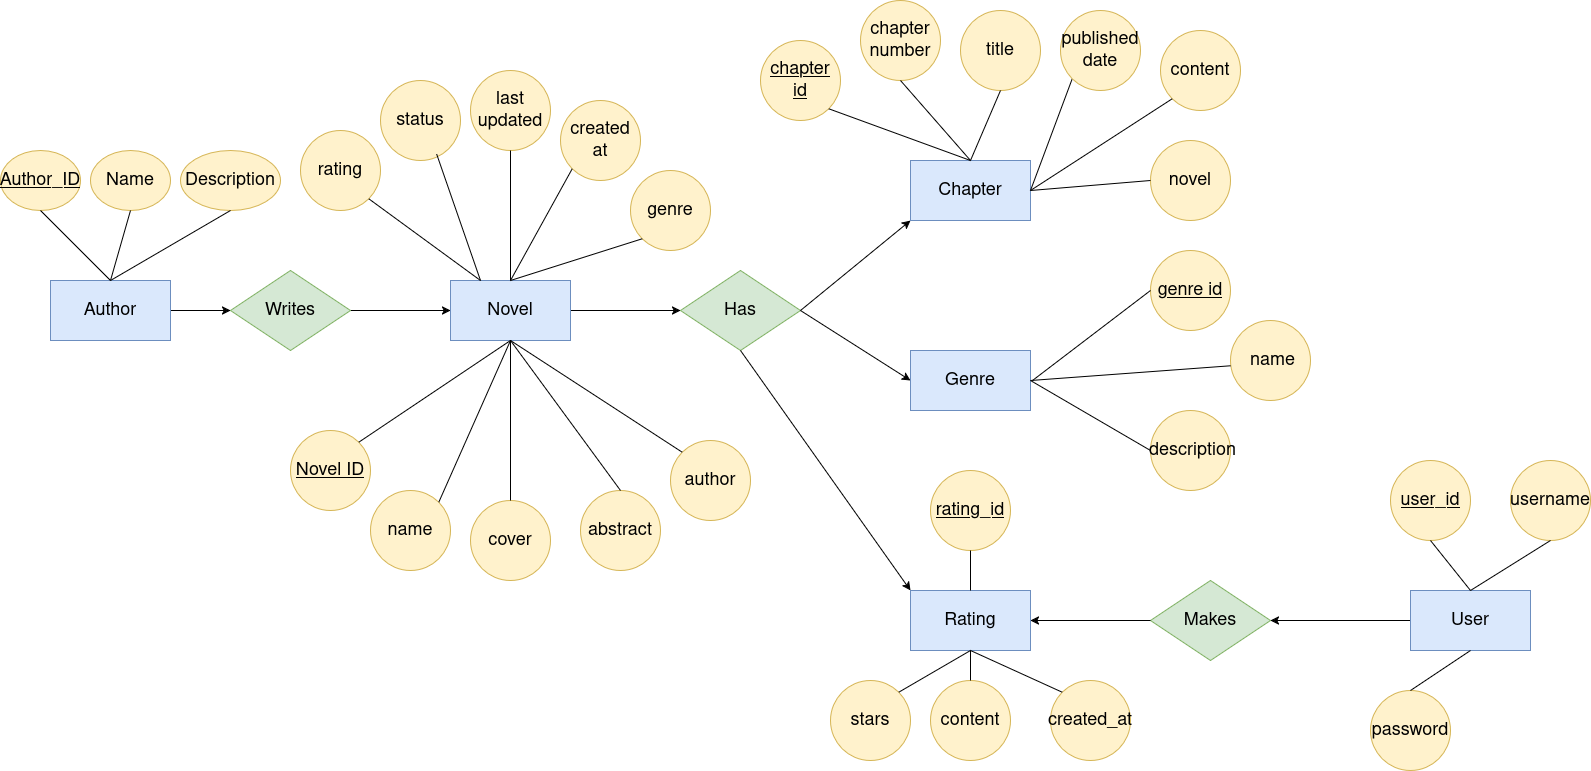
\includegraphics[width=0.8\textwidth]{img/ER.png}
    \end{center}
\end{frame}

\section{Câu lệnh SQL}

\begin{frame}[fragile]
\frametitle{Bảng auth\_user (Người dùng hệ thống)}
\begin{lstlisting}[language=SQL, basicstyle=\small\ttfamily]
-- Django's built-in User table (simplified)
CREATE TABLE auth_user (
    id INTEGER PRIMARY KEY AUTOINCREMENT,
    username VARCHAR(150) UNIQUE NOT NULL,
    first_name VARCHAR(150),
    last_name VARCHAR(150),
    email VARCHAR(254),
    is_staff BOOLEAN DEFAULT FALSE,
    is_active BOOLEAN DEFAULT TRUE,
    is_superuser BOOLEAN DEFAULT FALSE,
    date_joined DATETIME DEFAULT CURRENT_TIMESTAMP,
    last_login DATETIME NULL,
    password VARCHAR(128) NOT NULL
);
\end{lstlisting}
\end{frame}

% Slide 1: Author Table
\begin{frame}[fragile]
\frametitle{Bảng Author (Tác giả)}
\begin{lstlisting}[language=SQL, basicstyle=\small\ttfamily]
CREATE TABLE Author (
    author_id INTEGER PRIMARY KEY AUTOINCREMENT,
    author_name VARCHAR(255) NOT NULL,
    description TEXT DEFAULT 'The author has not disclosed any information about themselves.',
    profile_picture VARCHAR(255) NULL
);
\end{lstlisting}
\end{frame}

% Slide 2: Genre Table
\begin{frame}[fragile]
\frametitle{Bảng Genre (Thể loại)}
\begin{lstlisting}[language=SQL, basicstyle=\small\ttfamily]
CREATE TABLE Genre (
    genre_id INTEGER PRIMARY KEY AUTOINCREMENT,
    genre_name VARCHAR(100) NOT NULL,
    genre_description TEXT NOT NULL
);
\end{lstlisting}
\end{frame}

% Slide 3: Novel Table
\begin{frame}[fragile,allowframebreaks]
\frametitle{Bảng Novel (Tiểu thuyết)}
\begin{lstlisting}[language=SQL, basicstyle=\small\ttfamily]
CREATE TABLE Novel (
    novel_id INTEGER PRIMARY KEY AUTOINCREMENT,
    name VARCHAR(255) NOT NULL,
    description TEXT NOT NULL,
    cover VARCHAR(255) NULL,
    status VARCHAR(50) DEFAULT 'ongoing' 
        CHECK (status IN ('ongoing', 'completed', 'hiatus', 'dropped')),
    last_updated DATETIME DEFAULT CURRENT_TIMESTAMP,
    created_at DATETIME DEFAULT CURRENT_TIMESTAMP
);
\end{lstlisting}
\end{frame}

% Slide 4: Novel-Author Relationship
\begin{frame}[fragile]
\frametitle{Bảng quan hệ Novel-Author (Tiểu thuyết - Tác giả)}
\begin{lstlisting}[language=SQL, basicstyle=\small\ttfamily]
-- Many-to-Many relationship table
CREATE TABLE Novel_Authors (
    id INTEGER PRIMARY KEY AUTOINCREMENT,
    novel_id INTEGER NOT NULL,
    author_id INTEGER NOT NULL,
    FOREIGN KEY (novel_id) REFERENCES Novel(novel_id),
    FOREIGN KEY (author_id) REFERENCES Author(author_id),
    UNIQUE(novel_id, author_id)
);
\end{lstlisting}
\end{frame}

% Slide 5: Novel-Genre Relationship
\begin{frame}[fragile]
\frametitle{Bảng quan hệ Novel-Genre (Tiểu thuyết - Thể loại)}
\begin{lstlisting}[language=SQL, basicstyle=\small\ttfamily]
-- Many-to-Many relationship table
CREATE TABLE Novel_Genres (
    id INTEGER PRIMARY KEY AUTOINCREMENT,
    novel_id INTEGER NOT NULL,
    genre_id INTEGER NOT NULL,
    FOREIGN KEY (novel_id) REFERENCES Novel(novel_id),
    FOREIGN KEY (genre_id) REFERENCES Genre(genre_id),
    UNIQUE(novel_id, genre_id)
);
\end{lstlisting}
\end{frame}

% Slide 5.5: Trigger for updating last_updated
\begin{frame}[fragile]
\frametitle{Trigger: Cập nhật last\_updated khi có thay đổi}
\begin{lstlisting}[language=SQL, basicstyle=\small\ttfamily]
CREATE TRIGGER update_last_updated
AFTER INSERT OR UPDATE ON Chapter
BEGIN
    UPDATE Novel
    SET last_updated = CURRENT_TIMESTAMP
    WHERE novel_id = NEW.novel_id;
END;
\end{lstlisting}
\end{frame}

% Slide 6: Chapter Table
\begin{frame}[fragile]
\frametitle{Bảng Chapter (Chương)}
\begin{lstlisting}[language=SQL, basicstyle=\small\ttfamily]
CREATE TABLE Chapter (
    chapter_id INTEGER PRIMARY KEY AUTOINCREMENT,
    novel_id INTEGER NOT NULL,
    chapter_number INTEGER NOT NULL,
    title VARCHAR(255) NOT NULL,
    published_date DATETIME DEFAULT CURRENT_TIMESTAMP,
    content TEXT NOT NULL,
    FOREIGN KEY (novel_id) REFERENCES Novel(novel_id),
    UNIQUE(novel_id, chapter_number)
    -- Ensure chapter_number is unique within a novel
);
\end{lstlisting}
\end{frame}

% Slide 7: Rating Table
\begin{frame}[fragile]
\frametitle{Bảng Rating (Đánh giá)}
\begin{lstlisting}[language=SQL, basicstyle=\small\ttfamily]
CREATE TABLE Rating (
    rating_id INTEGER PRIMARY KEY AUTOINCREMENT,
    novel_id INTEGER NOT NULL,
    user_id INTEGER NOT NULL,
    stars INTEGER NOT NULL CHECK (stars BETWEEN 1 AND 5),
    content TEXT NULL,
    created_at DATETIME DEFAULT CURRENT_TIMESTAMP,
    FOREIGN KEY (novel_id) REFERENCES Novel(novel_id),
    FOREIGN KEY (user_id) REFERENCES auth_user(id),
    UNIQUE(novel_id, user_id)
);
\end{lstlisting}
\end{frame}

% Slide 8: Query - Tìm tác giả theo tên
\begin{frame}[fragile]
\frametitle{Truy vấn: Tìm tác giả theo tên}
\begin{lstlisting}[language=SQL, basicstyle=\small\ttfamily]
-- Find authors by name pattern
SELECT author_id, author_name, description 
FROM Author 
WHERE author_name LIKE '%Nguyen%';

-- Get all authors with their profile pictures
SELECT author_name, description, profile_picture
FROM Author 
WHERE profile_picture IS NOT NULL
ORDER BY author_name;
\end{lstlisting}
\end{frame}

% Slide 9: Query - Lấy thông tin thể loại
\begin{frame}[fragile]
\frametitle{Truy vấn: Lấy thông tin thể loại}
\begin{lstlisting}[language=SQL, basicstyle=\small\ttfamily]
-- Get all genres ordered by name
SELECT genre_name, genre_description 
FROM Genre 
ORDER BY genre_name;

-- Count novels in each genre
SELECT g.genre_name, COUNT(ng.novel_id) as novel_count
FROM Genre g
LEFT JOIN Novel_Genres ng ON g.genre_id = ng.genre_id
GROUP BY g.genre_id, g.genre_name
ORDER BY novel_count DESC;
\end{lstlisting}
\end{frame}

% Slide 10: Query - Lọc tiểu thuyết theo trạng thái
\begin{frame}[fragile]
\frametitle{Truy vấn: Lọc tiểu thuyết theo trạng thái}
\begin{lstlisting}[language=SQL, basicstyle=\small\ttfamily]
-- Get ongoing novels ordered by last update
SELECT name, status, last_updated 
FROM Novel 
WHERE status = 'ongoing' 
ORDER BY last_updated DESC;

-- Get completed novels with their creation date
SELECT name, description, created_at
FROM Novel 
WHERE status = 'completed'
ORDER BY created_at DESC;
\end{lstlisting}
\end{frame}

% Slide 10.5: Function to format author names
\begin{frame}[fragile]
\frametitle{Hàm: Định dạng tên tác giả}
\begin{lstlisting}[language=SQL, basicstyle=\footnotesize\ttfamily]
-- Create function to format author names
CREATE FUNCTION format_author_names(novel_id_param INTEGER)
RETURNS TEXT
READS SQL DATA
DETERMINISTIC
BEGIN
    DECLARE author_list TEXT DEFAULT '';
    
    SELECT GROUP_CONCAT(a.author_name SEPARATOR ', ') INTO author_list
    FROM Author a JOIN Novel_Authors na ON a.author_id = na.author_id
    WHERE na.novel_id = novel_id_param ORDER BY a.author_name;
    
    RETURN COALESCE(author_list, 'Unknown Author');
END;
\end{lstlisting}
\end{frame}

% Slide 11: Query - Lấy thông tin tác giả của tiểu thuyết
\begin{frame}[fragile, allowframebreaks]
\frametitle{Truy vấn: Lấy thông tin tác giả của tiểu thuyết}
\begin{lstlisting}[language=SQL, basicstyle=\small\ttfamily]
-- Get novels with their authors
SELECT n.name as novel_name, 
       format_author_names(n.novel_id) as authors, 
       n.status, 
       n.last_updated
FROM Novel n
JOIN Novel_Authors na ON n.novel_id = na.novel_id
JOIN Author a ON na.author_id = a.author_id
GROUP BY n.novel_id, n.name, n.status, n.last_updated
ORDER BY n.last_updated DESC, n.name;
\end{lstlisting}
\framebreak

\begin{lstlisting}[language=SQL, basicstyle=\small\ttfamily]
-- Get all novels by a specific author
SELECT n.name, n.status, n.last_updated
FROM Novel n
JOIN Novel_Authors na ON n.novel_id = na.novel_id
JOIN Author a ON na.author_id = a.author_id
WHERE a.author_name = 'Nguyen Van A';
\end{lstlisting}
\end{frame}

% Slide 12: Query - Lấy thể loại của tiểu thuyết
\begin{frame}[fragile]
\frametitle{Truy vấn: Lấy thể loại của tiểu thuyết}
\begin{lstlisting}[language=SQL, basicstyle=\small\ttfamily]
-- Get novels with their genres
SELECT n.name as novel_name, g.genre_name 
FROM Novel n
JOIN Novel_Genres ng ON n.novel_id = ng.novel_id
JOIN Genre g ON ng.genre_id = g.genre_id
ORDER BY n.name;

-- Get all Fantasy novels
SELECT n.name, n.description
FROM Novel n
JOIN Novel_Genres ng ON n.novel_id = ng.novel_id
JOIN Genre g ON ng.genre_id = g.genre_id
WHERE g.genre_name = 'Fantasy';
\end{lstlisting}
\end{frame}

% Slide 13: Query - Lấy chương của tiểu thuyết
\begin{frame}[fragile]
\frametitle{Truy vấn: Lấy chương của tiểu thuyết}
\begin{lstlisting}[language=SQL, basicstyle=\small\ttfamily]
-- Get chapters of a specific novel
SELECT chapter_number, title, published_date FROM Chapter 
WHERE novel_id = 1 
ORDER BY chapter_number;

-- Get latest chapter of each novel
SELECT n.name, c.title, c.published_date FROM Novel n
JOIN Chapter c ON n.novel_id = c.novel_id
WHERE c.published_date = (
    SELECT MAX(published_date) 
    FROM Chapter c2 
    WHERE c2.novel_id = n.novel_id
);
\end{lstlisting}
\end{frame}

% Slide 14: Query - Tính điểm đánh giá trung bình
\begin{frame}[fragile,allowframebreaks]
\frametitle{Truy vấn: Tính điểm đánh giá trung bình}
\begin{lstlisting}[language=SQL, basicstyle=\small\ttfamily]
-- Get average rating for each novel
SELECT n.name, 
       AVG(r.stars) as average_rating, 
       COUNT(r.rating_id) as total_ratings
FROM Novel n
LEFT JOIN Rating r ON n.novel_id = r.novel_id
GROUP BY n.novel_id, n.name
ORDER BY average_rating DESC;
\end{lstlisting}

\framebreak

\begin{lstlisting}[language=SQL, basicstyle=\small\ttfamily]
-- Get highly rated novels (4+ stars)
SELECT n.name, AVG(r.stars) as avg_rating FROM Novel n
JOIN Rating r ON n.novel_id = r.novel_id
GROUP BY n.novel_id, n.name
HAVING AVG(r.stars) >= 4.0
ORDER BY avg_rating DESC;
\end{lstlisting}
\end{frame}

% Slide 15: Query - Truy vấn phức tạp
\begin{frame}[fragile]
\frametitle{Truy vấn phức tạp: Lấy thông tin tiểu thuyết}
\begin{lstlisting}[language=SQL, basicstyle=\tiny\ttfamily]
-- Get detailed info: novels with authors, genres, avg rating, chapter count
SELECT 
    n.novel_id,
    n.name AS novel_name,
    n.status AS novel_status,
    GROUP_CONCAT(DISTINCT a.author_name) AS authors,
    GROUP_CONCAT(DISTINCT g.genre_name) AS genres,
    IFNULL(AVG(r.stars), 0) AS avg_rating,
    COUNT(DISTINCT c.chapter_id) AS chapter_count
FROM Novel n
LEFT JOIN Novel_Authors na ON n.novel_id = na.novel_id
LEFT JOIN Author a ON na.author_id = a.author_id
LEFT JOIN Novel_Genres ng ON n.novel_id = ng.novel_id
LEFT JOIN Genre g ON ng.genre_id = g.genre_id
LEFT JOIN Rating r ON n.novel_id = r.novel_id
LEFT JOIN Chapter c ON n.novel_id = c.novel_id
WHERE n.status IN ('ongoing', 'completed')
GROUP BY n.novel_id, n.name, n.status
ORDER BY n.last_updated DESC, n.name;
\end{lstlisting}
\end{frame}

% Slide 16: Query - Lấy tiểu thuyết đang hot
\begin{frame}[fragile]
\frametitle{Truy vấn: Lấy tiểu thuyết đang hot}
\begin{lstlisting}[language=SQL, basicstyle=\scriptsize\ttfamily]
-- Get trending novels (recent updates + high ratings)
SELECT 
    n.name, 
    n.status,
    AVG(r.stars) as avg_rating,
    COUNT(r.rating_id) as rating_count,
    n.last_updated,
    (AVG(r.stars) * (1.0 / (julianday('now') - julianday(n.last_updated) + 1))) 
    as trending_score
FROM Novel n
LEFT JOIN Rating r ON n.novel_id = r.novel_id
WHERE n.status IN ('ongoing', 'completed')
GROUP BY n.novel_id, n.name, n.status, n.last_updated
HAVING COUNT(r.rating_id) > 0
ORDER BY trending_score DESC
LIMIT 10;
\end{lstlisting}
\end{frame}

% Slide 17: A better way for trending novels
\begin{frame}[fragile,allowframebreaks]
\frametitle{Cách khác để lấy tiểu thuyết đang hot?}
\begin{lstlisting}[language=SQL, basicstyle=\footnotesize\ttfamily]
ALTER TABLE Novel
ADD COLUMN trending_score REAL DEFAULT 0;

CREATE TRIGGER update_trending_score
AFTER INSERT OR UPDATE ON Rating
BEGIN
    UPDATE Novel
    SET trending_score = (
        SELECT AVG(stars) * (1.0 / (julianday('now') - julianday(last_updated) + 1))
        FROM Rating
        WHERE novel_id = NEW.novel_id
    )
    WHERE novel_id = NEW.novel_id;
END;
\end{lstlisting}

\framebreak
\begin{lstlisting}[language=SQL, basicstyle=\small\ttfamily]
CREATE EVENT update_trending_score_event
ON SCHEDULE EVERY 1 DAY
DO
BEGIN
    UPDATE Novel
    SET trending_score = (
        SELECT AVG(stars) * (1.0 / (julianday('now') - julianday(last_updated) + 1))
        FROM Rating
        WHERE novel_id = Novel.novel_id
    );
END;
\end{lstlisting}

\framebreak
\begin{lstlisting}[language=SQL, basicstyle=\small\ttfamily]
-- Get top 10 trending novels
SELECT name, status, trending_score
FROM Novel
ORDER BY trending_score DESC
LIMIT 10;
\end{lstlisting}
\end{frame}

\end{document}
